\documentclass[10pt,a4paper]{article}
\usepackage[T1]{fontenc}\usepackage[utf8]{inputenc}\usepackage{lmodern,textcomp}
\usepackage[english]{babel}\babelprovide[import=fr]{french}\usepackage[a4paper,margin=21mm,headheight=14pt]{geometry}
\usepackage{amsmath,amssymb,mathtools,microtype,xcolor,graphicx,longtable,booktabs,array,needspace,fancyhdr,hyperref,tikz}
\usetikzlibrary{arrows.meta,positioning,calc}
\definecolor{ink}{HTML}{154C4C}\definecolor{paper}{HTML}{F0F5F3}
\hypersetup{colorlinks=true,linkcolor=ink,urlcolor=ink,pdftitle={GMT - Equations and code},pdfauthor={Romain VIALA}}
\pagestyle{fancy}\fancyhf{}\fancyhead[L]{\small\sffamily GMT}\fancyhead[R]{\small\sffamily 1.10.0 / FR + EN}\fancyfoot[L]{\small\sffamily Romain VIALA}\fancyfoot[R]{\thepage}
\setlength{\parindent}{0pt}\setlength{\parskip}{5pt}\setlength{\emergencystretch}{2em}
\newcommand{\FR}[1]{\textbf{FR.} #1\par}\newcommand{\EN}[1]{{\selectlanguage{english}\textbf{EN.} #1\par}}
\newcommand{\loc}[1]{{\small\color{ink}\textbf{Code :} #1\par}}
\newcommand{\sinc}{\operatorname{sinc}}\newcommand{\clip}{\operatorname{clip}}\newcommand{\diag}{\operatorname{diag}}\newcommand{\Rea}{\operatorname{Re}}\newcommand{\rms}{\operatorname{RMS}}
\allowdisplaybreaks[2]
\begin{document}
{\sffamily\color{ink}\Huge GMT\par}\vspace{3mm}
{\sffamily\Large Équations et architecture du code\par Equations and code architecture\par}\vspace{5mm}
\textbf{Auteur des applications / Application author : Romain VIALA}\par
Version 1.10.0 · 3 novembre 2026 / 3 November 2026\par
\FR{Ce manuel décrit les équations physiques, numériques, acoustiques, statistiques et de traitement du signal de cette distribution. Les opérations de mise en page en pixels et les contrôles de formulaire sont exclus. Les paramètres illustratifs ne sont pas des mesures.}
\EN{This manual describes the physical, numerical, acoustic, statistical and signal-processing equations in this distribution. Pixel layout and form validation are excluded. Illustrative parameters are not measurements.}
\FR{Les renvois sont relatifs à la racine du dépôt et comptent les lignes à partir de 1. Une plage désigne le bloc de fonction qui implémente le groupe ; une ligne seule désigne l’ancre de code. Une ligne JavaScript compacte peut contenir plusieurs équations. Le code fait foi pour les bornes et détails d’implémentation. source-map.json contient les ancres et empreintes SHA-256 ; verify\_references.py détecte les modifications.}
\EN{References are relative to the repository root and use one-based lines. Ranges identify implementing function blocks; single lines identify code anchors. A compact JavaScript line may contain several equations. Code is authoritative for bounds and implementation details. source-map.json records anchors and SHA-256 hashes; verify\_references.py detects changes.}
\FR{Conventions : unités SI sauf mention contraire ; $f$ en Hz, $\omega=2\pi f$ en rad/s, $f_s$ fréquence d’échantillonnage, $t$ en s, $i^2=-1$. Gain d’amplitude $10^{g/20}$ pour g en dB ; $\sinc x=\sin x/x$, avec $\sinc0=1$.}
\EN{Conventions: SI unless stated otherwise; $f$ in Hz, $\omega=2\pi f$ in rad/s, sample rate $f_s$, time $t$ in seconds, $i^2=-1$. Amplitude gain $10^{g/20}$ for g in dB; $\sinc x=\sin x/x$, with $\sinc0=1$.}
\clearpage\tableofcontents\clearpage

\section{Modèles et équations / Models and equations}
\begin{samepage}\Needspace{9\baselineskip}\subsection{Tenseur orthotrope / Orthotropic tensor}
\loc{\texttt{backend/catalog.py} : 61-65}
\begin{align}\sigma&=C\varepsilon,\quad C=S^{-1},\quad S\succ0,\\
S_{ii}&=1/E_i\ (i=1,2,3),\quad (S_{44},S_{55},S_{66})=(1/G_{LR},1/G_{LT},1/G_{RT}),\\
S_{12}&=-\nu_{LR}/E_L,\quad S_{13}=-\nu_{LT}/E_L,\quad S_{23}=-\nu_{RT}/E_R,\\
S_{ij}&=S_{ji}.\end{align}
\FR{Ordre de Voigt LL, RR, TT, LR, LT, RT, avec cisaillements d’ingénieur. Les modules GPa deviennent des Pa par 1e9. La symétrie de souplesse impose la réciprocité des coefficients de Poisson. Une énergie non positive est rejetée.}
\EN{Voigt order is LL, RR, TT, LR, LT, RT with engineering shear. GPa converts to Pa by 1e9. Symmetric compliance enforces Poisson reciprocity. Nonpositive energy is rejected.}
\end{samepage}
\begin{samepage}\Needspace{9\baselineskip}\subsection{TET10 et quadrature / TET10 and quadrature}
\loc{\texttt{backend/fem.py} : 17-21}
\begin{align}N_i&=\lambda_i(2\lambda_i-1),\quad N_{ij}=4\lambda_i\lambda_j\ (i<j),\quad\sum_{i=1}^4\lambda_i=1,\\
x&=\sum_{a=1}^{10}N_ax_a,\quad J=\partial x/\partial\xi,\quad\nabla_xN=J^{-T}\nabla_\xi N,\\
K_e&=\int B^TCB\,dV,\qquad M_e=\rho\int N^TN\otimes I_3\,dV.\end{align}
\FR{Quatre sommets et six milieux d’arêtes. B calcule les déformations d’ingénieur ; la masse est cohérente. Quadrature à 11 points : centroïde (poids -0,0131555555555556), 4 permutations de (11/14,1/14,1/14,1/14), poids 0,00762222222222222 ; 6 permutations de (a,a,b,b), a=0,399403576166799, b=0,100596423833201, poids 0,0248888888888889. Somme des poids : 1/6.}
\EN{Four vertices and six edge midpoints. B computes engineering strain; mass is consistent. Eleven-point quadrature: centroid weight -74/5625; four permutations of (11/14,1/14,1/14,1/14) with weight 343/45000; six permutations of (a,a,b,b), where a=(1+sqrt(5/14))/4 and b=(1-sqrt(5/14))/4, with weight 28/1125. These are exact algorithm constants, not measured precision. Weights sum to 1/6.}
\end{samepage}
\begin{samepage}\Needspace{9\baselineskip}\subsection{Modes élastiques / Elastic modes}
\loc{\texttt{backend/fem.py} : 53-99}
\begin{align}K\phi_j&=\lambda_j M\phi_j,\quad\phi_i^TM\phi_j=\delta_{ij},\\
f_j&=\sqrt{\lambda_j}/(2\pi),\qquad r_j=\frac{\|K\phi_j-\lambda_jM\phi_j\|}{\max(\|K\phi_j\|,\epsilon)}.\end{align}
\FR{Solveur propre creux avec décalage spectral, retrait des degrés bloqués et des six mouvements rigides en libre-libre. La normalisation est massique. Un faible résidu ne garantit pas la convergence de maillage ; les modes hors bande ne justifient pas une extrapolation précise.}
\EN{Sparse shifted eigensolver, removal of constrained degrees and six free-free rigid modes. Normalization is mass-based. Low residual does not establish mesh convergence; out-of-band modes do not justify accurate extrapolation.}
\end{samepage}
\begin{samepage}\Needspace{9\baselineskip}\subsection{Contours de référence et pan coupé / Reference outlines and cutaway}
\loc{\texttt{backend/contours.py} : 16-17, 28-57, 59-77}
\begin{align}(x_j,y_j)&=(W u_j,L v_j),\\B(t)&=(1-t)^3P_0+3(1-t)^2tP_1+3(1-t)t^2P_2+t^3P_3,\\b(t)&=t^2(3-2t),\quad a\prime(t)=a(t)+(1-b)(N-a_0)+b(R-a_1).\end{align}
\FR{Les points normalisés (u,v) proviennent des données GMT 1.6 documentées dans CONTOURS.md. Les dimensions W,L converties en mètres donnent le contour. Il ne s’agit plus de demi-largeurs PCHIP originales. Le pan coupé s’adapte au talon N et à l’épaule R, puis sa profondeur varie avec un poids cosinus nul à la corne. Un raccord Bézier tangentiel rejoint le contour. Formes invalides ou aire inférieure à 65 \% refusées. Conditions de redistribution distinctes : PUBLICATION.md.}
\EN{Normalized (u,v) points are GMT 1.6 reference data documented in CONTOURS.md. Width W and length L in metres scale the outline. These are no longer original PCHIP half-widths. Cutaway adapts to neck N and shoulder R; depth follows a cosine weight ending at the horn, with a tangent Bézier join. Invalid shapes or area below 65\% are rejected. Separate content conditions: PUBLICATION.md.}
\end{samepage}
\begin{samepage}\Needspace{9\baselineskip}\subsection{Mise à l’échelle et voûte / Scaling and arch}
\loc{\texttt{backend/contours.py} : 59-77;\allowbreak\quad \texttt{backend/geometry.py} : 57-62, 64-67}
\begin{align}x'&=W[x-(x_{min}+x_{max})/2]/(x_{max}-x_{min}),\\
y'&=L(y-y_{min})/(y_{max}-y_{min}),\\
a(x,y)&=H\max[0,1-(2x/W)^2]\max[0,\sin(\pi y/L)]^{1.2},\\
z'&=z+t a_{top}-(1-t)a_{back},\quad t=\clip[(z+d)/d,0,1].\end{align}
\FR{L, W, H et d sont en m après conversion des entrées mm. Le contour importé est centré et redimensionné. La simplification est bornée par la distance de Hausdorff. La voûte déforme le maillage ; ce modèle paramétrique ne copie pas une table historique.}
\EN{L, W, H and d are meters after mm input conversion. Imported outline is centered and scaled. Simplification is bounded by Hausdorff distance. Arch warps the mesh; this parametric model does not copy a historical plate.}
\end{samepage}
\begin{samepage}\Needspace{9\baselineskip}\subsection{Rosace et ouïes / Soundhole and apertures}
\loc{\texttt{backend/geometry.py} : 12-25, 27-36, 38-43}
\begin{align}x(\theta)&=c_x+r_x\cos\theta,\quad y(\theta)=c_y+r_y\sin\theta,\\
p_{SVG}&=(width\,u+c_x,height\,v+c_y),\\
x_f(t)&=c_x\pm[0.21W+0.7r_x\sin(2\pi t)],\quad y_f(t)=c_y+r_y(2t-1).\end{align}
\FR{La largeur et la hauteur règlent la taille du trou de rosace. Le cercle/ellipse utilise 40 segments ; l’ouverture D est recoupée par un demi-plan. Les ouïes f sont des lignes épaissies de 0,32rx. Les contours SVG sont redimensionnés comme des ouvertures distinctes, contrôlées vis-à-vis des éclisses, du chevalet et entre elles.}
\EN{Width and height control soundhole size. Circle/ellipse uses 40 segments; D opening is clipped by a half-plane. f-holes are lines buffered by 0.32rx. SVG rings scale as separate apertures, checked against ribs, bridge and each other.}
\end{samepage}
\begin{samepage}\Needspace{9\baselineskip}\subsection{Transformations et courbes SVG / SVG transforms and curves}
\loc{\texttt{backend/svg\_holes.py} : 147-189, 27-43, 45-55, 57-76}
\begin{align}\widetilde p'&=T_1T_2\cdots T_n\widetilde p,\quad\widetilde p=(x,y,1)^T,\\
R(\phi)&=\begin{pmatrix}\cos\phi&-\sin\phi\\\sin\phi&\cos\phi\end{pmatrix},\quad p'=R(p-c)+c,\\
p_{ij}^{new}&=(p_i+p_{i+1})/2,\\
p(\theta)&=c+R(\phi)(r_x\cos\theta,r_y\sin\theta)^T,\\
\Delta\theta&=2\arccos[\clip(1-tol/\max(r_x,r_y),-1,1)].\end{align}
\FR{Matrices affines, rotations, translations, échelles et cisaillements sont composés dans l’ordre SVG. Les Bézier se subdivisent par de Casteljau jusqu’à la tolérance de corde et d’excès de polygone de contrôle, profondeur au plus 16. Les arcs elliptiques utilisent la conversion extrémités-centre SVG et un pas borné par la flèche ; au plus 4096 points. Le code lit uniquement la géométrie inerte, sans exécuter scripts ou liens externes.}
\EN{Affine matrices, rotations, translation, scale and skew compose in SVG order. Bézier uses de Casteljau subdivision until chord-distance and control-polygon excess meet tolerance, depth at most 16. Elliptic arcs use SVG endpoint-to-center conversion and sagitta-bounded step, at most 4096 points. Only inert geometry is read, with no script or external-link execution.}
\end{samepage}
\begin{samepage}\Needspace{9\baselineskip}\subsection{Repères locaux et pertes / Local frames and losses}
\loc{\texttt{backend/fem.py} : 23-44, 46-51, 53-99}
\begin{align}\varepsilon_{LRT}&=R^T\varepsilon R,\quad e_{LRT}=Qe,\quad C_{global}=Q^TCQ,\\
K_{loss}&=\sum_p\eta_p K_p,\quad\eta_j=\phi_j^TK_{loss}\phi_j/\omega_j^2,\quad\zeta_j=\eta_j/2.\end{align}
\FR{Le repère matériau suit chaque pièce, les orientations de fil/cernes et la voûte, avec orthonormalisation. La matrice de pertes additionne les rigidités pondérées des pièces ; les pertes modales sont leur projection massiquement normalisée.}
\EN{Material frame follows each component, grain/ring angles and arch, with orthonormalization. Loss matrix sums component stiffnesses weighted by loss; modal damping projects onto mass-normalized modes.}
\end{samepage}
\begin{samepage}\Needspace{9\baselineskip}\subsection{Ports mécaniques et surfaces / Mechanical ports and surfaces}
\loc{\texttt{backend/fem.py} : 102-123, 125-139;\allowbreak\quad \texttt{backend/response.py} : 12-23}
\begin{align}N_i^\triangle&=\lambda_i(2\lambda_i-1),\quad N_{ij}^\triangle=4\lambda_i\lambda_j,\\
u_{port}&=B^Tu,\quad F_{nodes}=BF_{port},\quad P=\Phi^TB,\\
S_{face,j}&=A_{face}\,n\cdot\frac{u_{mid1,j}+u_{mid2,j}+u_{mid3,j}}3 .\end{align}
\FR{Douze ports représentent six cordes en directions normale et tangentielle. Interpolation et distribution de force utilisent les mêmes fonctions quadratiques. L’intégrale surfacique exacte d’un triangle quadratique donne zéro aux sommets et un tiers aux milieux ; elle produit le déplacement volumique des panneaux rayonnants.}
\EN{Twelve ports represent six strings in normal and tangential directions. Interpolation and force spreading use the same quadratic functions. Exact quadratic triangle area averaging gives zero vertex weights and one third at edge midpoints, yielding radiating panel volume displacement.}
\end{samepage}
\begin{samepage}\Needspace{9\baselineskip}\subsection{Acoustique interne TET4 / Internal TET4 acoustics}
\loc{\texttt{backend/fem.py} : 141-153, 155-166}
\begin{align}K^a_e&=V_e\nabla N_i\cdot\nabla N_j,\quad M^a_e=V_e(\mathbf1+I)/20,\\
K^a\psi_j&=k_j^2M^a\psi_j,\quad\omega^a_j=c k_j,\quad\psi_i^TM^a\psi_j=\delta_{ij},\\
C_{ja}&=\int_{\Gamma}\psi_a(n\cdot\phi_j)\,dS,\quad h_a=\langle\psi_a\rangle_{hole}.\end{align}
\FR{La pression utilise des fonctions linéaires et la structure des fonctions quadratiques. Le couplage de surface est intégré sur les triangles avec six points de quadrature. Les modes acoustiques, dont le mode uniforme, interagissent avec la structure et les coordonnées d’ouverture.}
\EN{Pressure uses linear functions and structure quadratic ones. Surface coupling uses six-point triangle quadrature. Acoustic modes, including uniform mode, interact with structure and aperture coordinates.}
\end{samepage}
\begin{samepage}\Needspace{9\baselineskip}\subsection{Correction statique et modes résiduels / Static residual modes}
\loc{\texttt{backend/reduction.py} : 11-46}
\begin{align}K X&=B,\quad R=X-\Phi\Omega^{-2}\Phi^TB,\\
R&\leftarrow R-\Phi\Phi^TMR,\quad R^TKR=U\Lambda U^T,\quad Q=RU\Lambda^{-1/2},\\
Q^TKQz&=\lambda Q^TMQz,\\
\epsilon_{stat}&=\frac{\|P^T\Omega^{-2}P+P_r^T\Lambda_r^{-1}P_r-B^TX\|}{\|B^TX\|}.\end{align}
\FR{En libre-libre, la résolution statique utilise un système selle avec les six mouvements rigides massiquement orthogonaux. L’orthogonalisation est répétée deux fois ; les petites valeurs d’énergie sont supprimées. La base résiduelle complète les ports mais ne rend pas exact le modèle à fréquence arbitrairement haute.}
\EN{Free-free static solve uses a saddle system with six mass-orthogonal rigid motions. Orthogonalization repeats twice and small energy eigenvalues are removed. Residual basis completes port response but does not make the model exact at arbitrarily high frequency.}
\end{samepage}
\begin{samepage}\Needspace{9\baselineskip}\subsection{Ouverture acoustique et Helmholtz / Aperture and Helmholtz}
\loc{\texttt{backend/response.py} : 35-68, 82-91}
\begin{align}r_{eq}&=\sqrt{S/\pi},\quad\ell_{end}=a_{end}r_{eq},\quad M_h=\rho_a\ell_{end}/S,\\
R_h&=r_{factor}\left[\frac{\rho_a\omega^2}{4\pi c}+0.05M_h\max\left(1,c\sqrt{S/(V\ell_{end})}\right)\right],\\
d_h&=-\omega^2M_h+i\omega R_h,\\
f_H^{display}&=\frac{c}{2\pi}\sqrt{\frac S{V(t_{top}+a_{end}r_{eq})}}.\end{align}
\FR{Le solveur utilise une masse d’ouverture basée sur la correction d’extrémité, avec une résistance approchée. Le repère de Helmholtz affiché ajoute l’épaisseur de table et suppose une cavité rigide ; il ne remplace pas la solution couplée. Ne pas confondre ces deux longueurs effectives.}
\EN{The solver uses aperture mass based on end correction and approximate resistance. The displayed Helmholtz guide adds top thickness and assumes a rigid cavity; it does not replace the coupled solution. These two effective lengths must not be conflated.}
\end{samepage}
\begin{samepage}\Needspace{9\baselineskip}\subsection{Résolution vibroacoustique / Vibroacoustic solve}
\loc{\texttt{backend/response.py} : 25-33, 70-80}
\begin{align}d_j&=\omega_j^2-\omega^2+2i\omega\zeta_j\omega_j,\\
d_a&=k_a^2-(\omega/c)^2+2i\zeta_a\omega\omega_a/c^2,\quad\zeta_a=0.025,\\
D&=\diag(d_j,d_h),\quad A=\begin{bmatrix}C\\h\end{bmatrix},\quad q_0=D^{-1}F,\\
W&=\diag(d_a/(\rho_a\omega^2))-A^TD^{-1}A,\\
a&=W^{-1}A^Tq_0,\quad q=q_0+D^{-1}Aa,\quad Y=i\omega P^Tq.\end{align}
\FR{Ce complément de Schur élimine les variables mécaniques dans l’espace réduit puis restitue les coordonnées de structure et d’ouverture. Les modifications de pic multiplient les projections émettrice et réceptrice par 10\textasciicircum{}(gain/40). DC est traité séparément.}
\EN{This Schur complement eliminates mechanical variables in reduced space, then recovers structure and aperture coordinates. Peak edits multiply both emitting and receiving projections by 10\textasciicircum{}(gain/40). DC is treated separately.}
\end{samepage}
\begin{samepage}\Needspace{9\baselineskip}\subsection{Rayonnement extérieur / Exterior radiation}
\loc{\texttt{backend/response.py} : 35-68, 70-80}
\begin{align}G(d,\omega)&=e^{-i\omega d/c}/d,\\
H_{pF}&=-\frac{\rho_a\omega^2}{4\pi}\left[\sum_sG(d_s,\omega)S_s q_s+G(d_h,\omega)q_h\right].\end{align}
\FR{Somme de panneaux monopoles avec propagation vers le point d’écoute. La distance est bornée à 3 cm. Le rayonnement extérieur est approché et n’est pas un calcul BEM complet avec retour de charge acoustique. La pression simulée n’est pas une calibration de microphone.}
\EN{Monopole-panel sum propagates toward the listening point. Distance is bounded at 3 cm. Exterior radiation is approximate, not full BEM with radiation-loading feedback. Simulated pressure is not microphone calibration.}
\end{samepage}
\begin{samepage}\Needspace{9\baselineskip}\subsection{Corde : accordage et pertes / String tuning and loss}
\loc{\texttt{backend/strings.py} : 10-13, 5-8}
\begin{align}L&=L_0 2^{-r/12},\quad f_o=f_{A4}2^{(m-69)/12},\\
T&=4\mu L_0^2f_o^2-\pi^2EI/L_0^2,\\
f_0&=\frac1{2\pi}\sqrt{[T(\pi/L)^2+EI(\pi/L)^4]/\mu},\\
\alpha(f)&=loss+hf\,f+2\,10^{-8}f^2+palm(12+0.015f).\end{align}
\FR{Mu est saisi en g/m puis converti en kg/m. La tension négative est refusée. Les pertes de contact de paume sont phénoménologiques ; elles ne résolvent pas un contact non linéaire main-corde.}
\EN{Mu is entered in g/m and converted to kg/m. Negative tension is rejected. Palm losses are phenomenological, not a nonlinear hand-string contact solution.}
\end{samepage}
\begin{samepage}\Needspace{9\baselineskip}\subsection{Impédance de corde raide / Stiff-string impedance}
\loc{\texttt{backend/strings.py} : 15-20}
\begin{align}\omega_c&=\omega-i\alpha,\quad\Delta=\sqrt{T^2+4EI\mu\omega_c^2},\\
k^2&=\frac{2\mu\omega_c^2}{T+\Delta},\quad\kappa^2=\frac{T+\Delta}{2EI},\quad A=\frac{\kappa^2}{\kappa^2+k^2},\quad B=1-A,\\
D_s&=(T+EI k^2)k\cot(kL)A-EI k^2\kappa\coth(\kappa L)B,\\
Z_s&=D_s/(i\omega).\end{align}
\FR{La forme de k² évite une soustraction mal conditionnée. Pour EI négligeable, D=T k cot(kL), k=oméga\_c racine(mu/T). À DC le code impose Z=0. Cette impédance passive représente la charge mécanique de la corde au chevalet.}
\EN{The k² form avoids ill-conditioned subtraction. Negligible EI gives D=T k cot(kL), k=omega\_c sqrt(mu/T). Code sets Z=0 at DC. This passive impedance represents bridge string loading.}
\end{samepage}
\begin{samepage}\Needspace{9\baselineskip}\subsection{Charge couplée et passivité / Coupled loading and passivity}
\loc{\texttt{backend/response.py} : 82-91;\allowbreak\quad \texttt{backend/audio.py} : 27-67}
\begin{align}Q&=[I+\diag(Z_s)Y]^{-1},\quad Y_{loaded}=YQ,\quad H_{loaded}=HQ,\\
F&=QF_{blocked},\quad v=YF,\quad p=HF,\\
Y_H&=(Y+Y^*)/2,\quad\lambda_{min}(Y_H)\geq0\ \text{for passivity}.\end{align}
\FR{Les impédances de cordes chargent les douze ports ; les cordes non excitées peuvent rester actives pour la sympathie. La passivité est échantillonnée sur la grille, ce qui n’est pas une preuve continue sur toutes les fréquences.}
\EN{String impedances load twelve ports; unexcited strings can remain active for sympathy. Passivity is sampled on the frequency grid, not proven continuously at all frequencies.}
\end{samepage}
\begin{samepage}\Needspace{9\baselineskip}\subsection{Force bloquée, FFT et synthèse / Blocked force and synthesis}
\loc{\texttt{backend/audio.py} : 27-67, 69-75, 8-12}
\begin{align}q_n&=\frac{2F\sin(k_nx_p)}{L(Tk_n^2+EI k_n^4)}s_n^{exc},\\
F_b(t)&=\sum_n(Tk_n+EI k_n^3)q_n\cos(\omega_nt)e^{-\alpha_nt},\\
s_n^{exc}&=\sinc(k_nw/2)e^{-(1-hardness)f_n/f_h},\\
(F_z,F_x)&=F_b(\cos\theta,\sin\theta),\quad N=\mathrm{nextfast}(N_{audio}+2f_s).\end{align}
\FR{La force bloquée est celle d’une corde pincée à extrémité fixe, puis la résolution chargée donne force réelle, vitesse et pression. Le calcul FFT ajoute deux secondes de garde ; les transferts sont interpolés en parties réelle et imaginaire. Au-delà de la grille la décroissance est fmax/f. Les bords de bande sont adoucis ; cette méthode fréquentielle à durée finie reste une approximation transitoire.}
\EN{Blocked force comes from a fixed-end plucked string; loaded solve gives actual force, velocity and pressure. FFT adds two seconds of guard; transfer real and imaginary parts are interpolated. Beyond the grid decay is fmax/f. Band edges are tapered; finite-duration frequency-domain synthesis remains a transient approximation.}
\end{samepage}
\begin{samepage}\Needspace{9\baselineskip}\subsection{Phrases et tempo / Phrases and tempo}
\loc{\texttt{backend/repertoire.py} : 11-35;\allowbreak\quad \texttt{web/repertoire.js} : 15}
\begin{align}t_e&=60b_e/\mathrm{BPM},\quad L_{fret}=L_0 2^{-fret/12},\\
y_j&=\sum_e strength_e\,x_{string_e,fret_e}[j-\operatorname{round}(t_ef_s)]\,w_e[j].\end{align}
\FR{Les notes sont regroupées par corde/case afin de limiter la mémoire. Chaque attaque est une réponse linéaire indépendante utilisant les réglages de guitare. La fin de note reçoit un fondu de 15 ms. Les changements de doigté ne modélisent pas une interaction sympathique variant continûment dans le temps.}
\EN{Notes are grouped by string/fret to bound memory. Each attack is an independent linear response using current guitar settings. Note release receives a 15 ms fade. Finger changes do not model continuously time-varying sympathetic interaction.}
\end{samepage}
\begin{samepage}\Needspace{9\baselineskip}\subsection{Dispersion Monte-Carlo / Monte Carlo dispersion}
\loc{\texttt{backend/uncertainty.py} : 7-39}
\begin{align}\sigma&=\sqrt{\ln(1+CV^2)},\quad z=\sqrt{r}z_c+\sqrt{1-r}z_i,\\
a&=\exp(\sigma z-\sigma^2/2),\quad g_{dB}=40\log_{10}a,\\
(q_{10},q_{50},q_{90})&=\operatorname{quantile}_{0.1,0.5,0.9}|H^{(s)}(f)|.\end{align}
\FR{Les facteurs lognormaux ont une moyenne unitaire. La corrélation r partage un tirage commun au sein d’une famille de paramètres. Fréquences, pertes et gains sont perturbés avec bornes. Les quantiles point par point représentent la dispersion choisie, pas des intervalles de confiance expérimentaux ; les déformées, l’air et la base résiduelle restent fixés.}
\EN{Lognormal factors have unit mean. Correlation r shares a common draw within each parameter family. Frequencies, losses and gains are perturbed with bounds. Pointwise quantiles represent chosen dispersion, not experimental confidence intervals; mode shapes, air and residual basis remain fixed.}
\end{samepage}
\begin{samepage}\Needspace{9\baselineskip}\subsection{FFT et fenêtres spectrales / FFT and spectral windows}
\loc{\texttt{web/signal.js} : 2}
\begin{align}X_k&=\sum_{j=0}^{N-1}w_jx_je^{-2\pi i jk/N},\quad A_k=c_k|X_k|/\sum_jw_j,\\
L_k&=20\log_{10}\max(10^{-14},A_k),\quad a=2\pi j/(N-1),\\
w_H&=0.5-0.5\cos a,\quad w_{Ham}=0.54-0.46\cos a,\\
w_{Blackman}&=0.42-0.5\cos a+0.08\cos2a,\quad \Delta f=f_s/N.\end{align}
\FR{La FFT radix-2 impose une taille puissance de deux. Le spectre conserve N/2 bins ; le facteur ck vaut 1 à DC et 2 ailleurs. La fenêtre rectangulaire vaut un. Le zéro-remplissage ne crée pas de résolution physique supplémentaire.}
\EN{Radix-2 FFT requires power-of-two size. Spectrum retains N/2 bins; ck is 1 at DC and 2 elsewhere. Rectangular window is one. Zero padding does not create additional physical resolution.}
\end{samepage}
\begin{samepage}\Needspace{9\baselineskip}\subsection{Crête, RMS et WAV / Peak, RMS and WAV}
\loc{\texttt{web/signal.js} : 22}
\begin{align}P&=\max_j|x_j|,\quad x_{RMS}=\sqrt{N^{-1}\sum_jx_j^2},\\
q_{16}&=\operatorname{round}(s\,\clip(x,-1,1)),\quad s\in\{32767,32768\},\\
bytes_{data}&=N\,channels\,(bits/8),\quad byteRate=f_s\,channels\,(bits/8).\end{align}
\FR{PCM borne les échantillons à [-1,1]. Les variantes qui utilisent 32768 pour les valeurs négatives exploitent la plage signée complète ; GMT/ToneWood utilisent 32767 des deux côtés. Les conversions DataView sans arrondi explicite tronquent. Les WAV flottants, lorsqu’ils sont proposés, conservent les grandeurs physiques et leurs unités doivent être lues avec les métadonnées.}
\EN{PCM clips samples to [-1,1]. Variants using 32768 for negative values use the full signed range; GMT/ToneWood use 32767 on both sides. DataView conversion without explicit rounding truncates. Floating WAV, where offered, retains physical quantities whose units must be read with metadata.}
\end{samepage}
\begin{samepage}\Needspace{9\baselineskip}\subsection{Écoute et sélection spectrale / Monitoring and band selection}
\loc{\texttt{web/signal.js} : 23, 32, 41}
\begin{align}g_{req}&=v10^{g_{dB}/20}\begin{cases}0.8/P&\text{peak}\\0.12/RMS&\text{RMS}\\1&\text{physical}\end{cases},\\
g&=\min(g_{req},0.9/P),\\
w(f)&=\tfrac12[1+\cos(\pi d(f)/\Delta)]\quad(0<d<\Delta).\end{align}
\FR{Le gain d’écoute est plafonné par la crête. Une sélection temps-fréquence utilise une FFT avec 30 ms de garde, des transitions de 10 à 100 Hz et un fondu temporel de 5 ms. Les fenêtres graphiques min/max conservent les extrema des échantillons par bloc, sans filtrer les données physiques.}
\EN{Listening gain is peak-capped. Time-frequency selection uses FFT with 30 ms padding, 10-100 Hz transition width and 5 ms time fades. Graphical min/max envelopes retain block extrema without filtering physical data.}
\end{samepage}
\begin{samepage}\Needspace{9\baselineskip}\subsection{Précision affichée / Display precision}
\loc{\texttt{web/suite.js} : 13, 19}
\begin{align}d&=\lfloor\log_{10}u\rfloor-1,\quad h=10^d,\\x_{display}&=h\operatorname{round}(x/h),\quad u=\max(x-l,r-x).\end{align}
\FR{Affichage uniquement : trois chiffres significatifs en général, quatre au maximum pour les cotes et fréquences. Dans un intervalle FEMU [l,r], la plus grande demi-largeur u fixe le rang décimal de l’estimation et des deux bornes (deux chiffres significatifs de largeur). Aucun arrondi n’est appliqué aux calculs ni aux exports. Sans intervalle valide, format significatif standard. Les constantes algorithmiques exactes et numéros de lignes ne sont pas des mesures et restent complets.}
\EN{Display only: generally three significant digits, at most four for dimensions and frequencies. For FEMU interval [l,r], the larger half-width u determines the shared decimal place of the estimate and bounds (two significant digits in width). Calculations and exports are not rounded. Invalid intervals use standard significant formatting. Exact algorithm constants and line numbers are not measurements and retain full digits.}
\end{samepage}
\begin{samepage}\Needspace{9\baselineskip}\subsection{Échange modal Universal / Universal modal interchange}
\loc{\texttt{backend/universal.py} : 37-43, 6-35}
\begin{align}f_j&=\omega_j/(2\pi),\quad\zeta_j=\eta_j/2,\\\Phi_j^T M\Phi_j&=1,\quad n_{UFF}=n_{local}+1.\end{align}
\FR{UNV et UFF sont deux extensions du même format Universal ASCII. Export des modes secs EF d’origine, sans retouches virtuelles ni modes acoustiques. Données 164 : unités SI ; 2411 : tous les nœuds solides et coordonnées XYZ en mètres ; 2412 : peau triangulée pour visualisation, pas maillage volumique EF ; 55 : vecteurs réels XYZ normalisés en masse, fréquences Hz, amortissement visqueux équivalent eta/2. Identifiants locaux renumérotés de 1 à N. Le format standard E13.5 des données 55 conserve six chiffres significatifs ; le NPZ garde les tableaux numériques complets.}
\EN{UNV and UFF are two extensions of the same ASCII Universal format. Original dry FE modes are exported, without virtual modal edits or acoustic modes. Dataset 164: SI units; 2411: all solid nodes and XYZ coordinates in metres; 2412: triangular visualization skin, not a volume FE mesh; 55: real mass-normalized XYZ vectors, frequencies in Hz, equivalent viscous damping eta/2. Local node IDs are renumbered 1 through N. Dataset 55 standard E13.5 records retain six significant digits; NPZ keeps the complete numerical arrays.}
\end{samepage}
\clearpage\section{Arborescence / File tree}
\FR{Les groupes de fichiers correspondent aux modules actifs. Le manifeste CSV du dépôt donne la liste complète.}
\EN{File groups describe active modules. The repository CSV manifest lists every distributed file.}
\begin{center}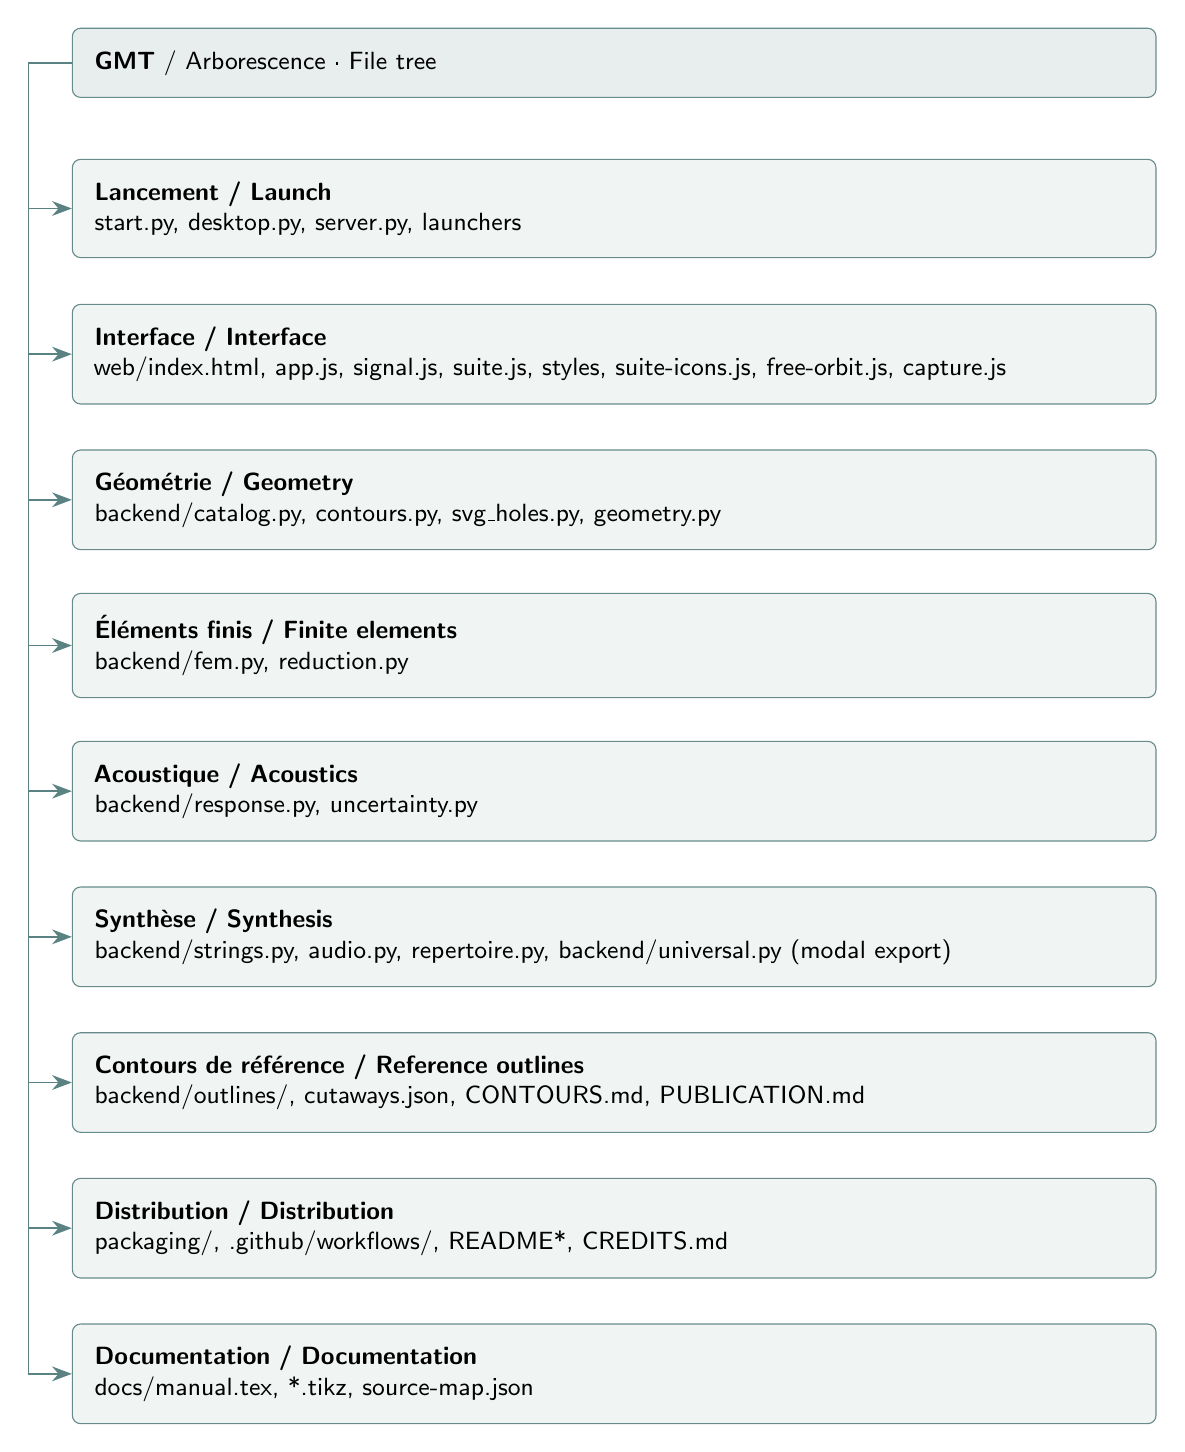
\begin{tikzpicture}[box/.style={draw=ink!65,fill=paper,rounded corners=3pt,align=left,text width=13.2cm,inner sep=8pt,font=\small\sffamily},arrow/.style={-{Stealth[length=2.5mm]},draw=ink!70,line width=.6pt}]

\node[box,fill=ink!10] (root) at (0,0) {\textbf{GMT} / Arborescence · File tree};
\node[box] (n1) at (0,-1.85) {\textbf{Lancement / Launch}\\ start.py, desktop.py, server.py, launchers};
\draw[arrow] (root.west) -- ++(-.55,0) |- (n1.west);
\node[box] (n2) at (0,-3.7) {\textbf{Interface / Interface}\\ web/index.html, app.js, signal.js, suite.js, styles, suite-icons.js, free-orbit.js, capture.js};
\draw[arrow] (root.west) -- ++(-.55,0) |- (n2.west);
\node[box] (n3) at (0,-5.550000000000001) {\textbf{Géométrie / Geometry}\\ backend/catalog.py, contours.py, svg\_holes.py, geometry.py};
\draw[arrow] (root.west) -- ++(-.55,0) |- (n3.west);
\node[box] (n4) at (0,-7.4) {\textbf{Éléments finis / Finite elements}\\ backend/fem.py, reduction.py};
\draw[arrow] (root.west) -- ++(-.55,0) |- (n4.west);
\node[box] (n5) at (0,-9.25) {\textbf{Acoustique / Acoustics}\\ backend/response.py, uncertainty.py};
\draw[arrow] (root.west) -- ++(-.55,0) |- (n5.west);
\node[box] (n6) at (0,-11.100000000000001) {\textbf{Synthèse / Synthesis}\\ backend/strings.py, audio.py, repertoire.py, backend/universal.py (modal export)};
\draw[arrow] (root.west) -- ++(-.55,0) |- (n6.west);
\node[box] (n7) at (0,-12.950000000000001) {\textbf{Contours de référence / Reference outlines}\\ backend/outlines/, cutaways.json, CONTOURS.md, PUBLICATION.md};
\draw[arrow] (root.west) -- ++(-.55,0) |- (n7.west);
\node[box] (n8) at (0,-14.8) {\textbf{Distribution / Distribution}\\ packaging/, .github/workflows/, README*, CREDITS.md};
\draw[arrow] (root.west) -- ++(-.55,0) |- (n8.west);
\node[box] (n9) at (0,-16.650000000000002) {\textbf{Documentation / Documentation}\\ docs/manual.tex, *.tikz, source-map.json};
\draw[arrow] (root.west) -- ++(-.55,0) |- (n9.west);
\end{tikzpicture}\end{center}
\clearpage\section{Interdépendances / Dependencies}
\FR{Flèches : appels, imports ou flux de données. Les sous-systèmes sont séparés pour garder les boîtes et les liens lisibles.}
\EN{Arrows: calls, imports or data flow. Subsystems are separated to keep boxes and links readable.}
\begin{center}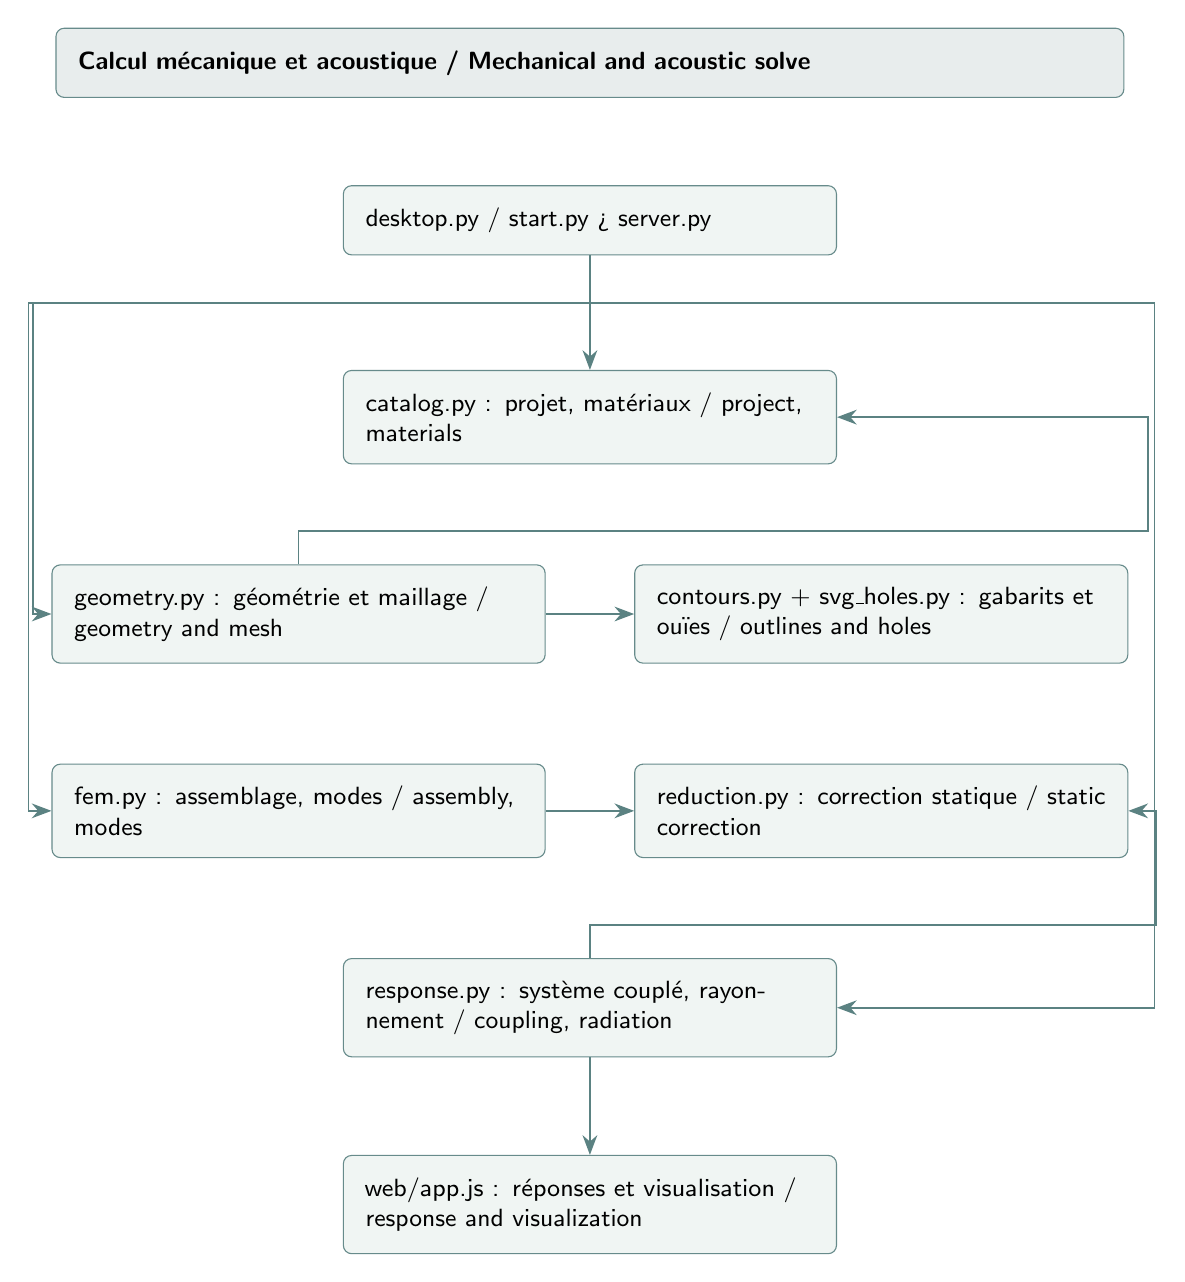
\begin{tikzpicture}[box/.style={draw=ink!65,fill=paper,rounded corners=3pt,align=left,text width=5.7cm,inner sep=8pt,font=\small\sffamily},arrow/.style={-{Stealth[length=2.5mm]},draw=ink!70,line width=.6pt}]

\node[box,text width=13cm,fill=ink!10] at (0,2) {\textbf{Calcul mécanique et acoustique / Mechanical and acoustic solve}};
\node[box] (n0) at (0,0) {desktop.py / start.py  >  server.py};
\node[box] (n1) at (0,-2.5) {catalog.py : projet, matériaux / project, materials};
\node[box] (n2) at (-3.7,-5) {geometry.py : géométrie et maillage / geometry and mesh};
\node[box] (n3) at (3.7,-5) {contours.py + svg\_holes.py : gabarits et ouïes / outlines and holes};
\node[box] (n4) at (-3.7,-7.5) {fem.py : assemblage, modes / assembly, modes};
\node[box] (n5) at (3.7,-7.5) {reduction.py : correction statique / static correction};
\node[box] (n6) at (0,-10) {response.py : système couplé, rayonnement / coupling, radiation};
\node[box] (n7) at (0,-12.5) {web/app.js : réponses et visualisation / response and visualization};
\draw[arrow] (n0.south) -- (n1.north);
\draw[arrow] (n0.south) -- (0,-1.05) -- (-7.069999999999999,-1.05) |- (n2.west);
\draw[arrow] (n2.north) -- (-3.7,-3.95) -- (7.09,-3.95) |- (n1.east);
\draw[arrow] (n2.east) -- (n3.west);
\draw[arrow] (n0.south) -- (0,-1.05) -- (-7.13,-1.05) |- (n4.west);
\draw[arrow] (n4.east) -- (n5.west);
\draw[arrow] (n0.south) -- (0,-1.05) -- (7.17,-1.05) |- (n6.east);
\draw[arrow] (n6.north) -- (0,-8.95) -- (7.1899999999999995,-8.95) |- (n5.east);
\draw[arrow] (n6.south) -- (n7.north);
\end{tikzpicture}
\newpage
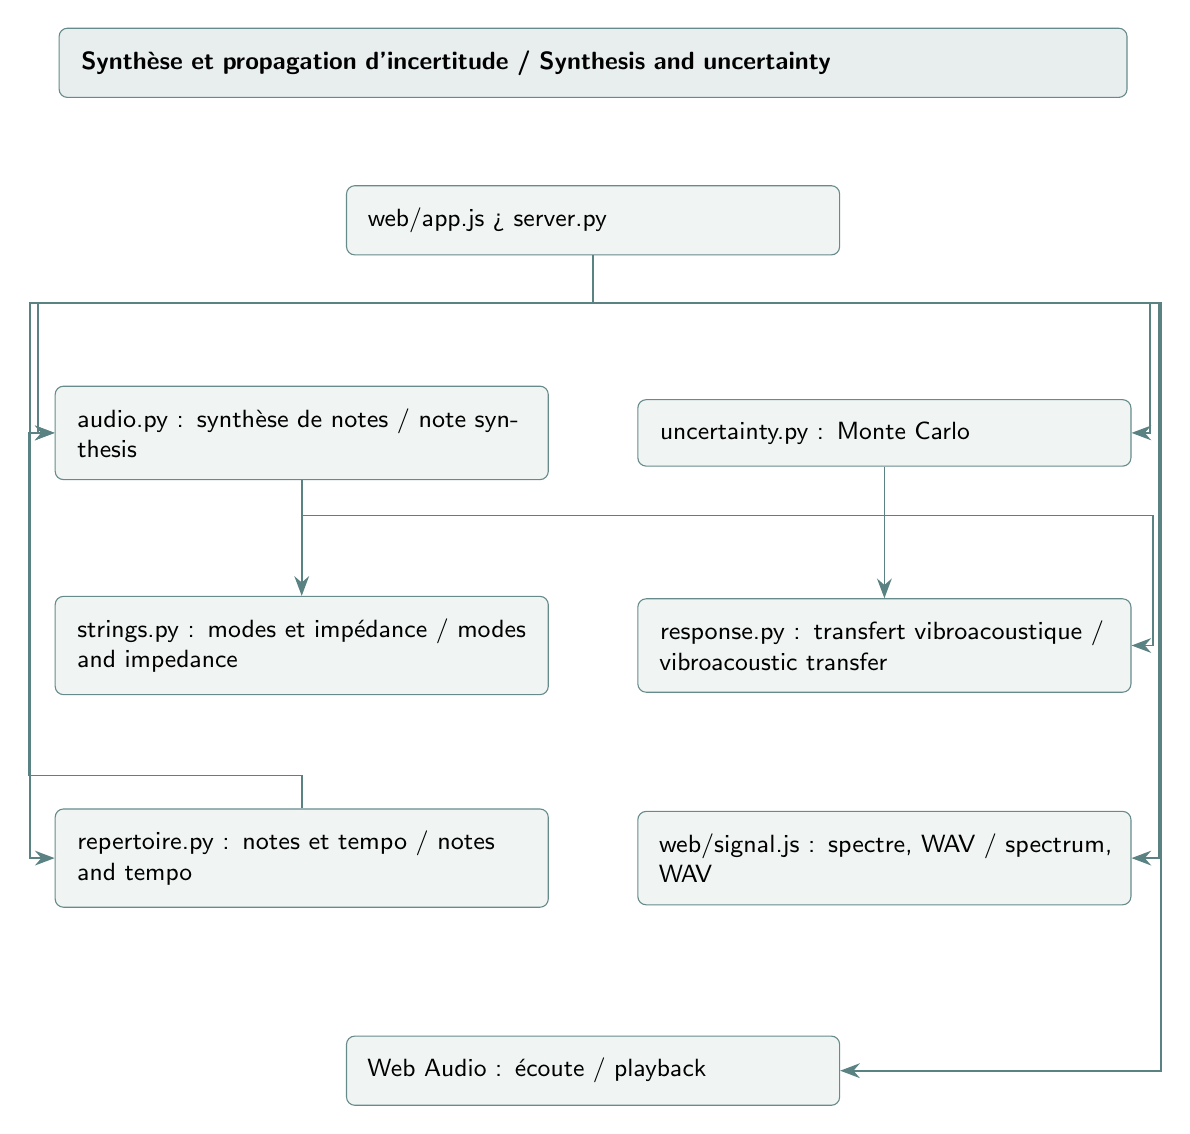
\begin{tikzpicture}[box/.style={draw=ink!65,fill=paper,rounded corners=3pt,align=left,text width=5.7cm,inner sep=8pt,font=\small\sffamily},arrow/.style={-{Stealth[length=2.5mm]},draw=ink!70,line width=.6pt}]

\node[box,text width=13cm,fill=ink!10] at (0,2) {\textbf{Synthèse et propagation d’incertitude / Synthesis and uncertainty}};
\node[box] (n0) at (0,0) {web/app.js  >  server.py};
\node[box] (n1) at (-3.7,-2.7) {audio.py : synthèse de notes / note synthesis};
\node[box] (n2) at (3.7,-2.7) {uncertainty.py : Monte Carlo};
\node[box] (n3) at (-3.7,-5.4) {strings.py : modes et impédance / modes and impedance};
\node[box] (n4) at (3.7,-5.4) {response.py : transfert vibroacoustique / vibroacoustic transfer};
\node[box] (n5) at (-3.7,-8.1) {repertoire.py : notes et tempo / notes and tempo};
\node[box] (n6) at (3.7,-8.1) {web/signal.js : spectre, WAV / spectrum, WAV};
\node[box] (n7) at (0,-10.8) {Web Audio : écoute / playback};
\draw[arrow] (n0.south) -- (0,-1.05) -- (-7.05,-1.05) |- (n1.west);
\draw[arrow] (n0.south) -- (0,-1.05) -- (7.069999999999999,-1.05) |- (n2.east);
\draw[arrow] (n1.south) -- (n3.north);
\draw[arrow] (n1.south) -- (-3.7,-3.75) -- (7.109999999999999,-3.75) |- (n4.east);
\draw[arrow] (n2.south) -- (n4.north);
\draw[arrow] (n0.south) -- (0,-1.05) -- (-7.1499999999999995,-1.05) |- (n5.west);
\draw[arrow] (n5.north) -- (-3.7,-7.05) -- (-7.17,-7.05) |- (n1.west);
\draw[arrow] (n0.south) -- (0,-1.05) -- (7.1899999999999995,-1.05) |- (n6.east);
\draw[arrow] (n0.south) -- (0,-1.05) -- (7.21,-1.05) |- (n7.east);
\end{tikzpicture}\end{center}
\clearpage\section{Index des équations / Equation index}
\small\begin{longtable}{p{8mm}p{75mm}p{65mm}}\toprule N° & Groupe / Group & Fichier, ligne / File, line \\ \midrule\endhead
1 & Tenseur orthotrope / Orthotropic tensor & \texttt{backend/catalog.py} : 61-65\\[3pt]
2 & TET10 et quadrature / TET10 and quadrature & \texttt{backend/fem.py} : 17-21\\[3pt]
3 & Modes élastiques / Elastic modes & \texttt{backend/fem.py} : 53-99\\[3pt]
4 & Contours de référence et pan coupé / Reference outlines and cutaway & \texttt{backend/contours.py} : 59-77\\[3pt]
4 & Contours de référence et pan coupé / Reference outlines and cutaway & \texttt{backend/contours.py} : 16-17\\[3pt]
4 & Contours de référence et pan coupé / Reference outlines and cutaway & \texttt{backend/contours.py} : 28-57\\[3pt]
5 & Mise à l’échelle et voûte / Scaling and arch & \texttt{backend/contours.py} : 59-77\\[3pt]
5 & Mise à l’échelle et voûte / Scaling and arch & \texttt{backend/geometry.py} : 57-62\\[3pt]
5 & Mise à l’échelle et voûte / Scaling and arch & \texttt{backend/geometry.py} : 64-67\\[3pt]
6 & Rosace et ouïes / Soundhole and apertures & \texttt{backend/geometry.py} : 12-25\\[3pt]
6 & Rosace et ouïes / Soundhole and apertures & \texttt{backend/geometry.py} : 27-36\\[3pt]
6 & Rosace et ouïes / Soundhole and apertures & \texttt{backend/geometry.py} : 38-43\\[3pt]
7 & Transformations et courbes SVG / SVG transforms and curves & \texttt{backend/svg\_holes.py} : 27-43\\[3pt]
7 & Transformations et courbes SVG / SVG transforms and curves & \texttt{backend/svg\_holes.py} : 45-55\\[3pt]
7 & Transformations et courbes SVG / SVG transforms and curves & \texttt{backend/svg\_holes.py} : 57-76\\[3pt]
7 & Transformations et courbes SVG / SVG transforms and curves & \texttt{backend/svg\_holes.py} : 147-189\\[3pt]
8 & Repères locaux et pertes / Local frames and losses & \texttt{backend/fem.py} : 23-44\\[3pt]
8 & Repères locaux et pertes / Local frames and losses & \texttt{backend/fem.py} : 46-51\\[3pt]
8 & Repères locaux et pertes / Local frames and losses & \texttt{backend/fem.py} : 53-99\\[3pt]
9 & Ports mécaniques et surfaces / Mechanical ports and surfaces & \texttt{backend/fem.py} : 125-139\\[3pt]
9 & Ports mécaniques et surfaces / Mechanical ports and surfaces & \texttt{backend/fem.py} : 102-123\\[3pt]
9 & Ports mécaniques et surfaces / Mechanical ports and surfaces & \texttt{backend/response.py} : 12-23\\[3pt]
10 & Acoustique interne TET4 / Internal TET4 acoustics & \texttt{backend/fem.py} : 141-153\\[3pt]
10 & Acoustique interne TET4 / Internal TET4 acoustics & \texttt{backend/fem.py} : 155-166\\[3pt]
11 & Correction statique et modes résiduels / Static residual modes & \texttt{backend/reduction.py} : 11-46\\[3pt]
12 & Ouverture acoustique et Helmholtz / Aperture and Helmholtz & \texttt{backend/response.py} : 35-68\\[3pt]
12 & Ouverture acoustique et Helmholtz / Aperture and Helmholtz & \texttt{backend/response.py} : 82-91\\[3pt]
13 & Résolution vibroacoustique / Vibroacoustic solve & \texttt{backend/response.py} : 25-33\\[3pt]
13 & Résolution vibroacoustique / Vibroacoustic solve & \texttt{backend/response.py} : 70-80\\[3pt]
14 & Rayonnement extérieur / Exterior radiation & \texttt{backend/response.py} : 35-68\\[3pt]
14 & Rayonnement extérieur / Exterior radiation & \texttt{backend/response.py} : 70-80\\[3pt]
15 & Corde : accordage et pertes / String tuning and loss & \texttt{backend/strings.py} : 5-8\\[3pt]
15 & Corde : accordage et pertes / String tuning and loss & \texttt{backend/strings.py} : 10-13\\[3pt]
16 & Impédance de corde raide / Stiff-string impedance & \texttt{backend/strings.py} : 15-20\\[3pt]
17 & Charge couplée et passivité / Coupled loading and passivity & \texttt{backend/response.py} : 82-91\\[3pt]
17 & Charge couplée et passivité / Coupled loading and passivity & \texttt{backend/audio.py} : 27-67\\[3pt]
18 & Force bloquée, FFT et synthèse / Blocked force and synthesis & \texttt{backend/audio.py} : 8-12\\[3pt]
18 & Force bloquée, FFT et synthèse / Blocked force and synthesis & \texttt{backend/audio.py} : 27-67\\[3pt]
18 & Force bloquée, FFT et synthèse / Blocked force and synthesis & \texttt{backend/audio.py} : 69-75\\[3pt]
19 & Phrases et tempo / Phrases and tempo & \texttt{backend/repertoire.py} : 11-35\\[3pt]
19 & Phrases et tempo / Phrases and tempo & \texttt{web/repertoire.js} : 15\\[3pt]
20 & Dispersion Monte-Carlo / Monte Carlo dispersion & \texttt{backend/uncertainty.py} : 7-39\\[3pt]
21 & FFT et fenêtres spectrales / FFT and spectral windows & \texttt{web/signal.js} : 2\\[3pt]
22 & Crête, RMS et WAV / Peak, RMS and WAV & \texttt{web/signal.js} : 22\\[3pt]
23 & Écoute et sélection spectrale / Monitoring and band selection & \texttt{web/signal.js} : 23\\[3pt]
23 & Écoute et sélection spectrale / Monitoring and band selection & \texttt{web/signal.js} : 41\\[3pt]
23 & Écoute et sélection spectrale / Monitoring and band selection & \texttt{web/signal.js} : 32\\[3pt]
24 & Précision affichée / Display precision & \texttt{web/suite.js} : 13\\[3pt]
24 & Précision affichée / Display precision & \texttt{web/suite.js} : 19\\[3pt]
25 & Échange modal Universal / Universal modal interchange & \texttt{backend/universal.py} : 6-35\\[3pt]
25 & Échange modal Universal / Universal modal interchange & \texttt{backend/universal.py} : 37-43\\[3pt]
\bottomrule\end{longtable}\normalsize
\Needspace{16\baselineskip}\section{Compilation et limites / Build and limitations}
\FR{Depuis docs/, exécuter deux fois pdflatex -halt-on-error manual.tex. Les fichiers *-standalone.tex compilent chaque schéma séparément. Papier A4, marges de 21 mm, sans réduction automatique des schémas. Les sources, licences et crédits tiers figurent dans CREDITS.md et SOURCES.md. Cette documentation décrit l’implémentation ; elle ne constitue pas une validation expérimentale.}
\EN{From docs/, run pdflatex -halt-on-error manual.tex twice. The *-standalone.tex wrappers compile each diagram separately. A4 paper, 21 mm margins, no automatic diagram shrinkage. Third-party sources, licenses and credits are in CREDITS.md and SOURCES.md. This documents implementation, not experimental validation.}
\end{document}